\documentclass[10pt,a4paper,british]{book}
\usepackage[T1]{fontenc}
\usepackage[utf8]{inputenc}
\usepackage{array}
\usepackage{color}
\usepackage{graphicx}

\makeatletter

%%%%%%%%%%%%%%%%%%%%%%%%%%%%%% LyX specific LaTeX commands.
%% Because html converters don't know tabularnewline
\providecommand{\tabularnewline}{\\}

\usepackage{amsmath}
\usepackage{amsfonts}
\usepackage{graphicx} 
\usepackage{amssymb}
\usepackage{calc,layouts}
\usepackage{titlesec}
\usepackage{fancyhdr}
\usepackage{xspace}
\usepackage{color}
\usepackage{ifthen}
\usepackage{boxedminipage}
\usepackage{lastpage}
\usepackage{setspace}
\usepackage{float}
\usepackage{afterpage}
\usepackage[german,british]{babel}

\setlength\textheight{240mm}
\setlength\textwidth{150mm}
\setlength\evensidemargin{15mm}
\setlength\oddsidemargin{15mm}
\setlength\topmargin{-15mm}
\setlength\headheight{15mm}
\setlength\parindent{0mm}
\setlength\parskip{2mm}

\usepackage[T1]{fontenc}
\usepackage[scaled]{helvet}
\renewcommand*\familydefault{\sfdefault}
\linespread{1.3}\selectfont

\titleformat{\chapter}{\LARGE \bf}{\hspace{-20mm}\parbox[b]{20mm}{\thechapter}}{0mm}{}
\titleformat{\section}{\Large \bf}{\hspace{-20mm}\parbox[b]{20mm}{\thesection}}{0mm}{}
\titleformat{\subsection}{\large \bf}{\hspace{-20mm}\parbox[b]{20mm}{\thesubsection}}{0mm}{}
\titleformat{\subsubsection}{\bf}{\hspace{-20mm}\parbox[b]{20mm}{\thesubsubsection}}{0mm}{}

\newcommand\engitsversion{draft}
\newcommand\engitsauthor{Author}
\newcommand\engitstitle{Title}
\newcommand\engitsdate{\today}
\newcommand\engitscopyright{Copyright by enGits GmbH}
\newcommand\setengitsversion[1]{\renewcommand\engitsversion{#1}}
\newcommand\setengitstitle[1]{\renewcommand\engitstitle{#1}}
\newcommand\setengitsauthor[1]{\renewcommand\engitsauthor{#1}}
\newcommand\setengitsdate[1]{\renewcommand\engitsdate{#1}}
\newcommand\setengitscopyright[1]{\renewcommand\engitscopyright{#1}}
\newcommand\eg{ENGRID\ }
\newcommand\foam{OpenFOAM\textsuperscript{\textregistered}\ }
\newcommand\netgen{NETGEN\ }
\newcommand\egv{1.0}
\newcommand\sqt{\char`\"{}}
\newcommand\eqt{\char`\"{}\ }
\newcommand\arr{\guillemotright\ }
\newcommand\menu[1]{\textcolor{blue}{\it \hspace{5mm} #1}}


\newcommand\makeengitstitle[1]
{
  \pagestyle{empty}
  \setengitstitle{#1}
  
  \hspace{0mm}
  \begin{minipage}[t]{130mm}
    {
      \vspace{3mm}
      \begin{center}
        
\includegraphics[width=75mm]{logos/titlelogo.png}
        $~$\\
        \vspace{10mm}
        \large
        \begin{tabular}{l}
          \begin{tabular}{l}
            \vspace{-1mm} enGits GmbH\\
            \vspace{-1mm} Marie-Curie-Strae 8\\
            \vspace{-1mm} 79539 Lrrach\\
            \vspace{0mm} Germany\\
          \end{tabular}\\
          \begin{tabular}{lcl}
            \vspace{-1mm} phone & : & +49 (0)7621 5500 530 \\
            \vspace{-1mm} fax & : & +49 (0)7621 5500 539 \\
            \vspace{-1mm} email & : & info@engits.com \\
          \end{tabular}\\
        \end{tabular}
        \vspace{3mm}$~$\\
      \end{center}
    }
  \end{minipage}
  
  \begin{minipage}[c][100mm][c]{130mm}
    \begin{center}
      {
        \begin{spacing}{1.5}
          \bf 
          \huge 
          \engitstitle
        \end{spacing}
      }
    \end{center}
  \end{minipage}
  \\
  \begin{minipage}{130mm}
    \begin{center}
      \begin{tabular}{|p{3cm}|p{81mm}|}
        \hline
        title & \engitstitle \\
        \hline
        date & \engitsdate \\
        \hline
        author & \engitsauthor \\
        \hline
        document-version & \engitsversion \\
        \hline
      \end{tabular}
    \end{center}
  \end{minipage}
  \clearpage
  \begin{minipage}{130mm}
    \begin{flushleft}
      {\engitscopyright}
    \end{flushleft}
  \end{minipage}
  \clearpage
  \pagestyle{fancy}

  \pagenumbering{roman}
  \tableofcontents
  \cleardoublepage
  \pagenumbering{arabic}
}

\newenvironment{engitsstandard}{}{\setlength\parskip{2mm}}
\newenvironment{engitstoc}{\setlength\parskip{0mm}}{\setlength\parskip{2mm}}

\pagestyle{fancy}
\fancyhf{}
\fancyhfoffset{0mm}
\fancyhfoffset[LO,LE]{20mm}
\fancyhead[LE,RO]{
  
\includegraphics[width=50mm]{logos/titlelogo.png}
}
\fancyhead[LO]{\rightmark}
\fancyhead[RE]{\leftmark}
\fancyfoot[LE,RO]{\thepage}

\definecolor{darkred}{rgb}{0.5,0,0}
\newcommand\important[1]
{
  $~$\\
  \begin{minipage}{15mm}
    
\includegraphics[width=1cm]{figures/important}
  \end{minipage}
  \begin{minipage}{110mm}
    \begin{flushleft}
      {\textcolor{darkred}{#1}}
    \end{flushleft}
  \end{minipage}
  \\
  \vspace{3mm}
}

\makeatother

\usepackage{babel}

\usepackage{rcs}
\RCS $Revision: 1.4 $

% floating stuff ///
% 
\setcounter{topnumber}{1}
\setcounter{bottomnumber}{1}
\renewcommand{\topfraction}{0.8}
\renewcommand{\bottomfraction}{0.8}
\renewcommand{\textfraction}{0.5}
\newcommand{\flush}{\afterpage{\clearpage}}



\begin{document}


\selectlanguage{british}
\setengitsauthor{O. Gloth}
\setengitsversion{CVS-\RCSRevision}


\setengitscopyright{Copyright \copyright 2008 enGits GmbH.\\
Permission is granted to copy, distribute and/or modify this document under the terms of the GNU Free Documentation License, Version~1.2 or any later version published by the Free Software Foundation; with
no Invariant Sections, no Front-Cover Texts, and no Back-Cover Texts. A copy of the license is included in the section entitled \char`\"{}GNU~Free~Documentation~License\char`\"{}.}


\makeengitstitle{enGrid manual}

\chapter{Introduction}

\eg is an open-source mesh generation software with CFD applications in mind. \eg uses the NETGEN \cite{netgen:2008} library for tetrahedral grid generation and an in-house development for prismatic boundary layer grids. Internally, \eg uses the VTK \cite{vtk:2008} data structures as well as the {*}.vtu file format. To create grids for
Currently \eg cannot generate surface grids. In order to create a volume grid it is required to import an existing surface mesh. Gmsh \cite{gmsh:2008} is an excellent open-source tool to create surface triangulations for \eg. Gmsh is able to import STEP and IGES files and it can also be used for simple geometry modelling. 

The \egv release of \eg provides native export to OpenFOAM\textsuperscript{\textregistered}\footnote{\foam is a registered trade mark of OpenCFD\textregistered Limited}\cite{openfoam:2008}. For future releases, export capabilities for complete \foam cases (including boundary conditions) and support for polyhedral cells are planned as well.

\eg is released under the GPL and we hope that it is a useful addition to the open-source CFD community. So far the implemented algorithm proved to be quite robust and it does not require much user interaction. Figure \ref{fig:Introduction1}shows a boundary layer grid that has been created around the geometry of what could be a toy plane.

\important
{
  This manual is very much a work in progress and does
  not claim to be finished, comprehensive, complete, or anything else.
  We hope that, even in this early stage, it offers a little help while
  using \eg!
}


\begin{figure}
\begin{centering}
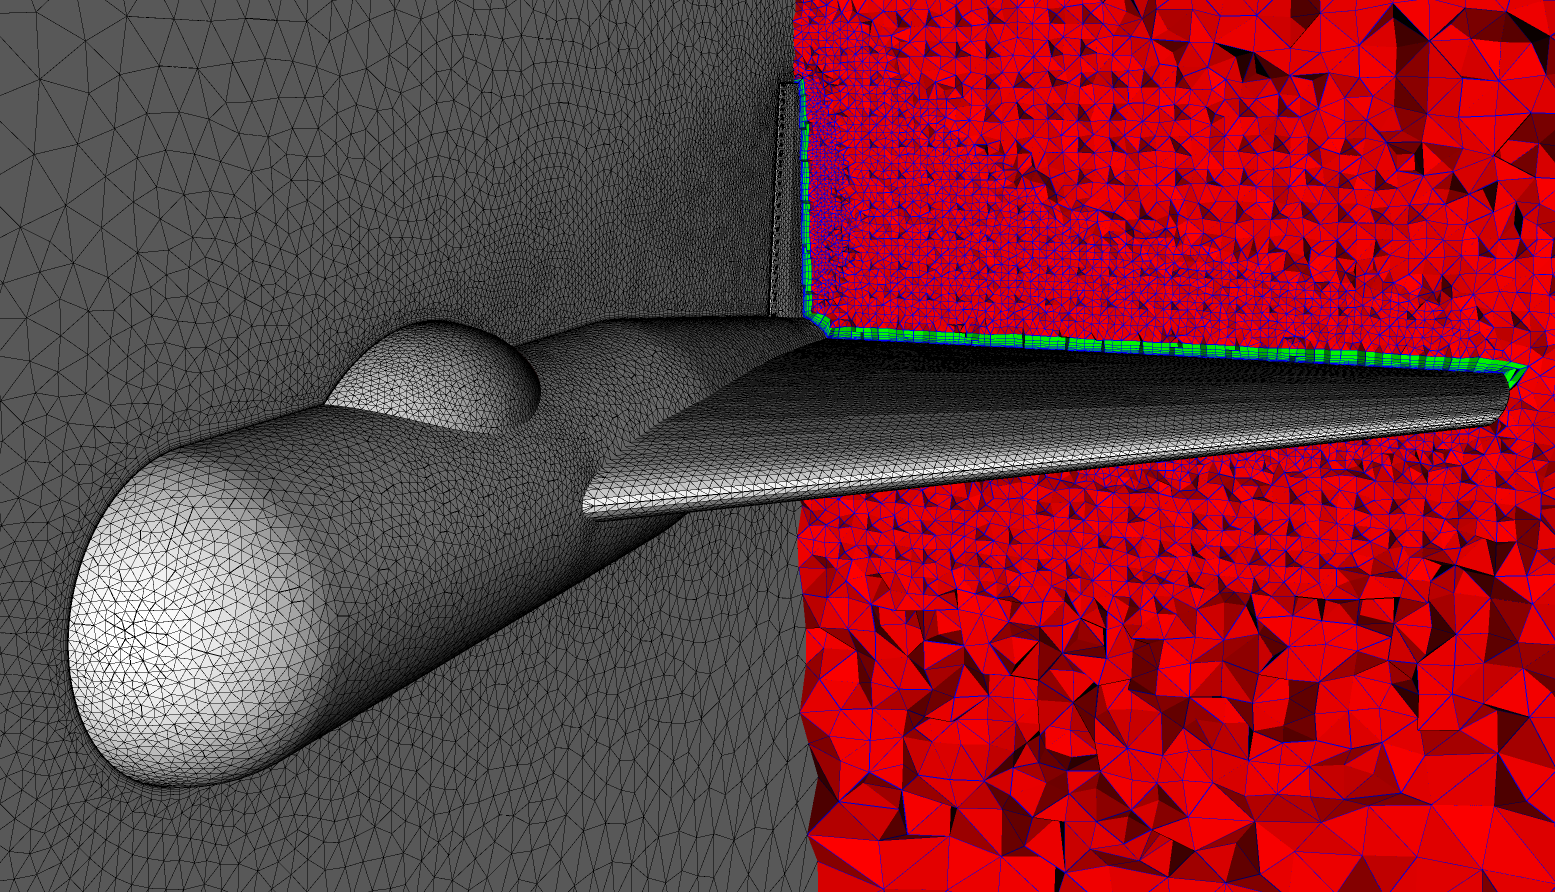
\includegraphics[width=7cm]{figures/DeltaWing_02}
\hspace{2mm}
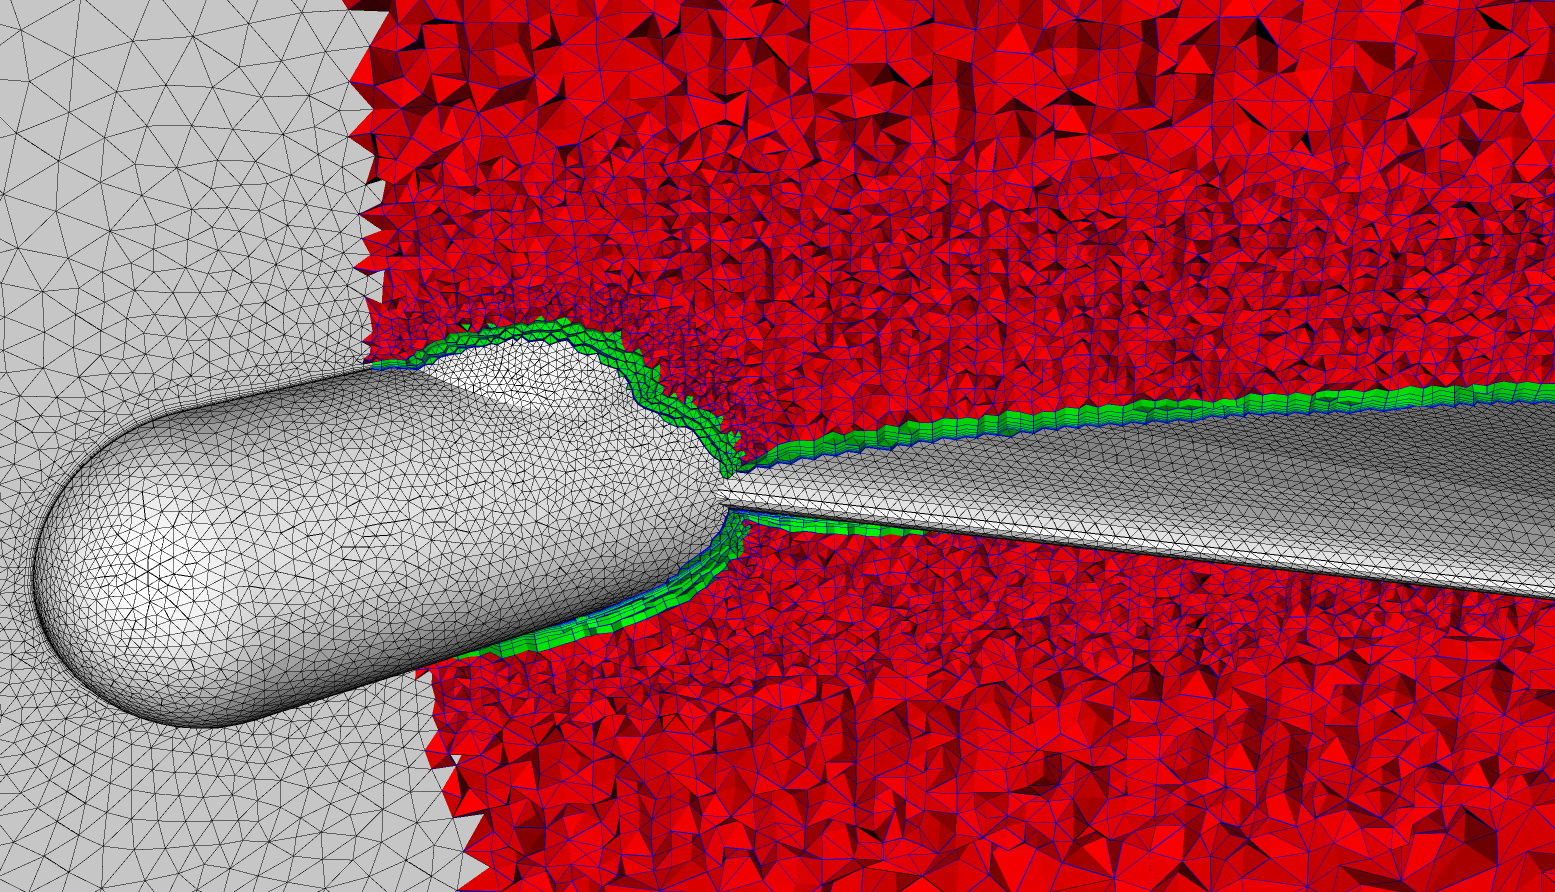
\includegraphics[width=7cm]{figures/DeltaWing_01}\\
\end{centering}
\caption{Prismatic boundary layer created by \eg}
\label{fig:Introduction1}
\end{figure}

\section{Current Release (\egv)}

\begin{itemize}
\item volume grids from existing surface triangulations (no surface meshing
support yet, but planned for future releases)
\item prismatic boundary layer support
\item GUI based on Qt4
\item direct export to OpenFOAM
\item experimental support for polyhedral grids in OpenFOAM
\end{itemize}

\section{Supported Platforms}

\begin{itemize}
\item \eg is developed on a LINUX system (OpenSUSE 10.3), using Qt-4.4.1,
VTK 5.2, and an SVN snapshot of NETGEN.
\item A Windows executable for Windows-XP (32bit) is also available.
\end{itemize}

\section{Supported File Formats}

\begin{itemize}
\item VTK unstructured grids in XML format (\eg's native format)
\item VTK poly data in XML format (import)
\item legacy VTK files (import)
\item OpenFOAM (export)
\item Gmsh (import \& export)
\item STL (import \& export)
\item NETGEN neutral format (export)
\end{itemize}


\chapter{Using \eg}


\section{Compilation and Installation}


\subsection{\eg on a UNIX system}

\subsubsection{Requirements}
\eg requires Qt-4.X and VTK-5.X. We use Qt-4.4.1 and VTK-5.2 but \eg should also compile with earlier versions. Please report any problems to the mailing list. We would, however, also appreciate if you report success with other versions than the ones mentioned before.

\important{Please make sure that VTK is compiled with GUI support for Qt-4.}

\subsubsection{Compilation}
\eg uses Qt's qmake tool to provide a platform independent compilation
mechanism. The source distribution has the following structure:
\begin{itemize}
\item enGrid\_\egv
\begin{itemize}
\item math
\item netgen\_svn
\item resources
\end{itemize}
\end{itemize}
First of all, you'll need to set up the following environment variables:
\begin{itemize}
\item VTKLIBDIR : Directory containing the VTK libraries
\item VTKINCDIR : Directory containing the VTK header files
\end{itemize}

On Debian or Ubuntu:
\begin{verbatim}
  export VTKLIBDIR=/usr/lib/
  export VTKINCDIR=/usr/include/vtk-5.0/
\end{verbatim}

On OpenSUSE:
\begin{verbatim}
  export VTKLIBDIR=/usr/lib64
  export VTKINCDIR=/usr/include/vtk
\end{verbatim}

Then to compile \eg you need to first compile the NETGEN library. We have created a Qt project file and a shell script to simplify this. In the main source directory simply type \"{}./build-nglib.sh\"{}. This downloads the latest source code from NETGEN's SVN repository and compiles the necessary library. If this fails, please follow the instructions in the next paragraph.
Otherwise compile \eg with the following steps:
\begin{enumerate}
\item change into the main source directory
\item type qmake
\item type make
\end{enumerate}

\subsubsection{Compiling NETGEN release}
This paragraph is only of interest if the \"{}./build-nglib.sh\"{} command failed.
Download the latest stable release of NETGEN and place it in the \sqt netgen\_svn\eqt folder. The following steps should get you a working NETGEN library:
\begin{enumerate}
\item create a folder \sqt netgen\_svn/netgen-mesher\eqt
\item unpack the netgen-X.Y.Z.tar.gz file
\item move the folder \sqt netgen-X.Y.Z\eqt to \sqt netgen\_svn/netgen-mesher/netgen\eqt
\item change directory to \sqt netgen\_svn\eqt
\item type qmake 
\item type make
\end{enumerate}
After a successful compilation of the NETGEN library you can procede with the compilation of \eg as described in the previous paragraph.

\subsubsection{Installation}
There is no installation script yet. You can simply run \eg from the source directory by typing \sqt ./engrid\eqt or you copy the binary to a place where it will be found by the system (e.g. /usr/local/bin).

\subsection{Installing the Windows Binary}

This should, hopefully, be straightforward:
\begin{enumerate}
\item Download and save the installer 
\item Run the installer 
\item Start \eg
\end{enumerate}
Of course it is quite possible, if not even likely, that there are issues on certain systems. Please report any problems to the mailing list.

\clearpage

\section{Tutorials}

\subsection{Tutorial 1: Creating a First Mesh}

\begin{figure}
\begin{centering}
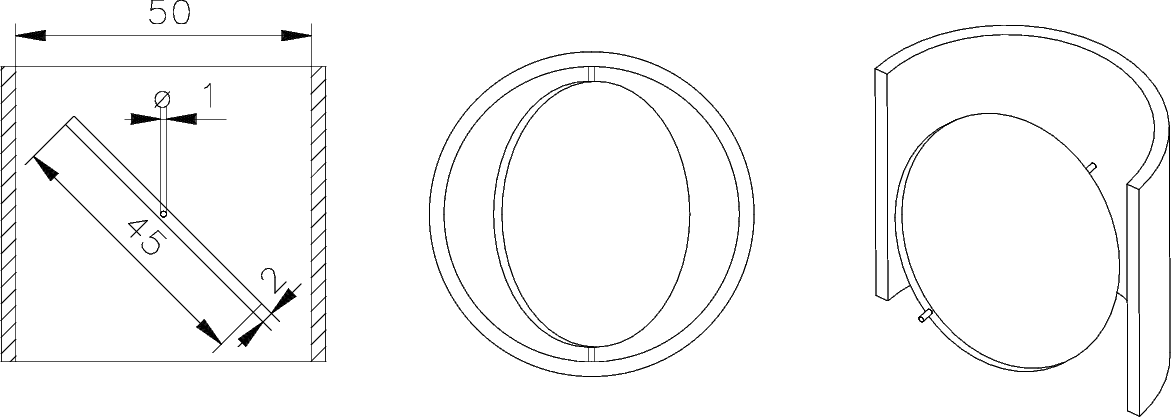
\includegraphics{figures/Throttle}
\par\end{centering}
\caption{Throttle geometry}
\label{fig:throttle1}
\end{figure}

\subsubsection{Description}

This tutorial will demonstrate how to read a surface mesh and create a volume mesh for a CFD simulation. Figure \ref{fig:throttle1}shows the geometry which will be used for this tutorial; it represents an adjustable throttle. The file containing the surface mesh for this tutorial is called \sqt Throttle.msh\eqt and it can be downloaded from the \eg download page. 

\subsubsection{Importing the Surface Mesh}
To start, please import the file choosing 

\menu{Import \arr Gmsh \arr v2.0 (ASCII)}

from the menu bar. A file-dialogue will show and you can browse for the file and open it. Figure \ref{fig:T1_scr01} shows a screen-shot of \eg after importing the file. You can use the mouse to rotate, move, and zoom the view. This mouse interaction is the default mouse interaction provided by VTK.

\eg colours the faces of the surface grid in order to determine which side of the surface is inside a flow domain and which is outside. The outside is coloured in a pale green, but figure \ref{fig:T1_scr01} shows pale yellow; this means the surface is wrongly oriented and it needs to be corrected. To do this, please choose 

\menu{Mesh \arr change surface orientation}

from the menu-bar. Afterwards the surface will be oriented correctly.


\begin{figure}
  \begin{centering}
    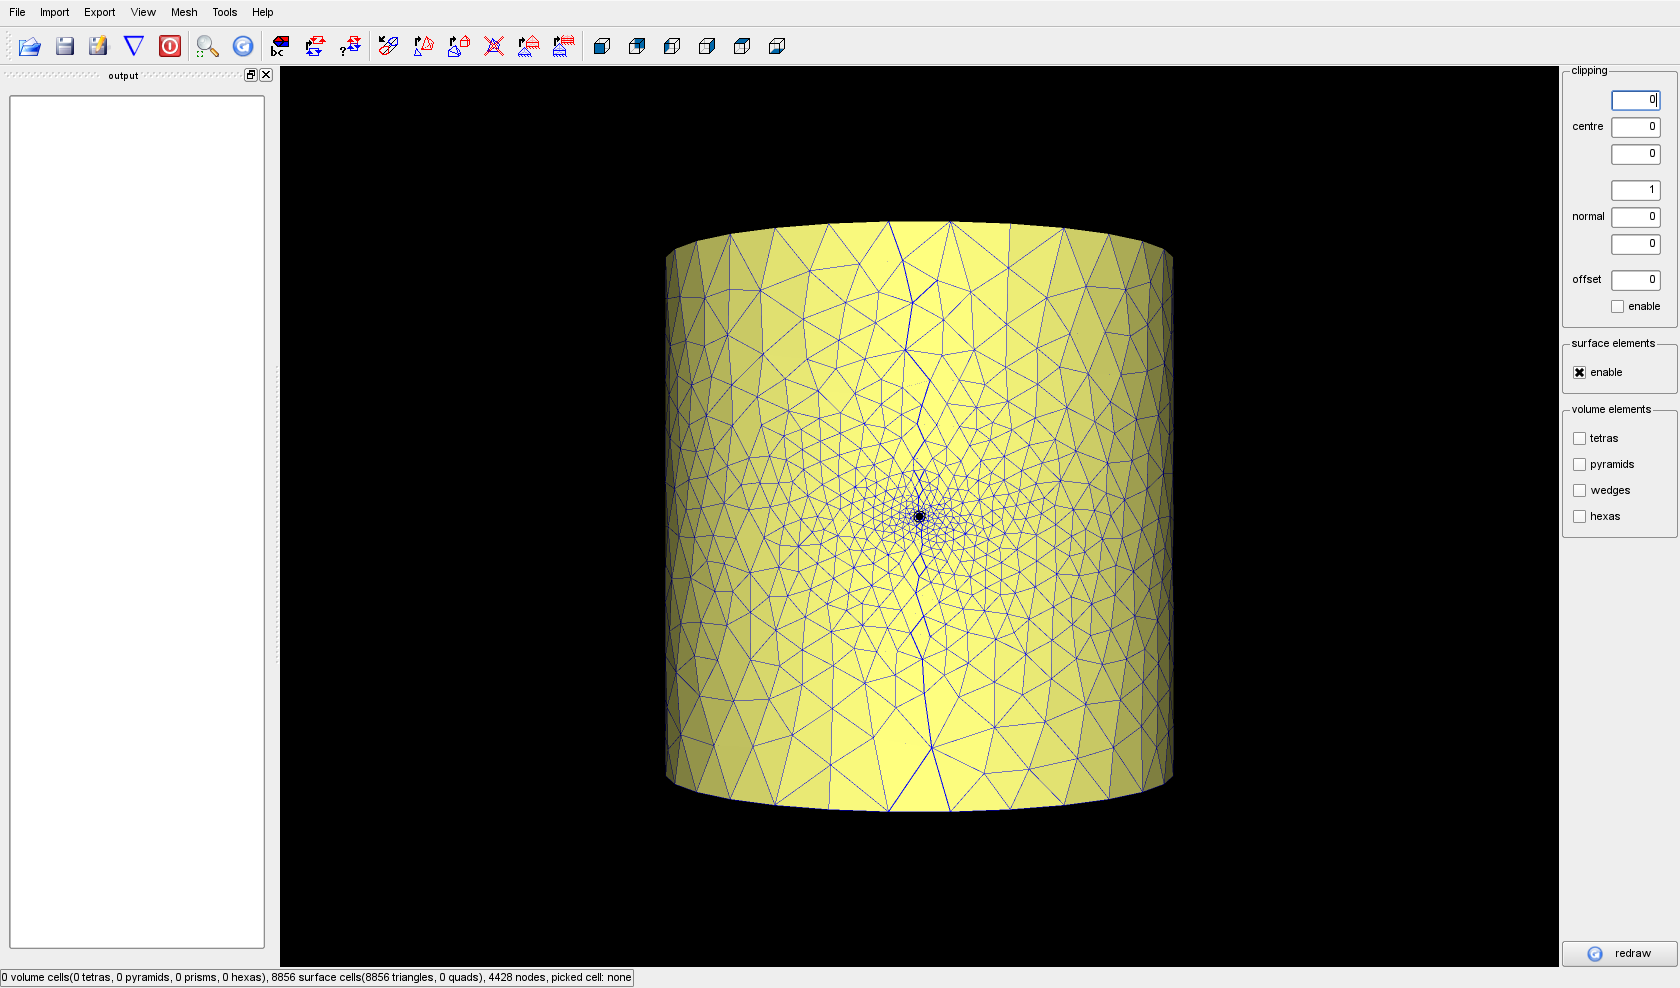
\includegraphics[width=14cm]{figures/tutorials/T1/scr01}
    \par
  \end{centering}
  \caption{After importing the surface mesh}
  \label{fig:T1_scr01}
\end{figure}

\subsubsection{Defining Boundary Conditions}
Unfortunately all faces belong to the same boundary condition and thus it is not possible to see inside the domain. To change this you can pick a surface on the side of the cylindrical geometry and then change its boundary condition to a different value. To pick a face, please point the mouse over a triangle and press the {}``P'' key on your keyboard. Afterwards you should see something similar to figure \ref{fig:T1_scr02}. To change the boundary code, please select 

\menu{Mesh \arr set boundary code}. 

A small dialogue will pop up and it offers to select a feature angle and a new boundary code. The new boundary code should be set to \sqt 2\eqt and the feature angle can remain at 45 degrees. With this setting you should set the whole side of the cylinder to a new boundary code and the faces should disappear, because they have not been selected for viewing yet. Now, do the same with the top (boundary condition 3) and the bottom (boundary condition 4) of the cylinder. To get rid of the red box, please point the mouse into an empty space and press {}``P'' again. Now would be a good time to save your work. Select 

\menu{File \arr Save Grid As}

to save the file. 

\begin{figure}
  \begin{centering}
    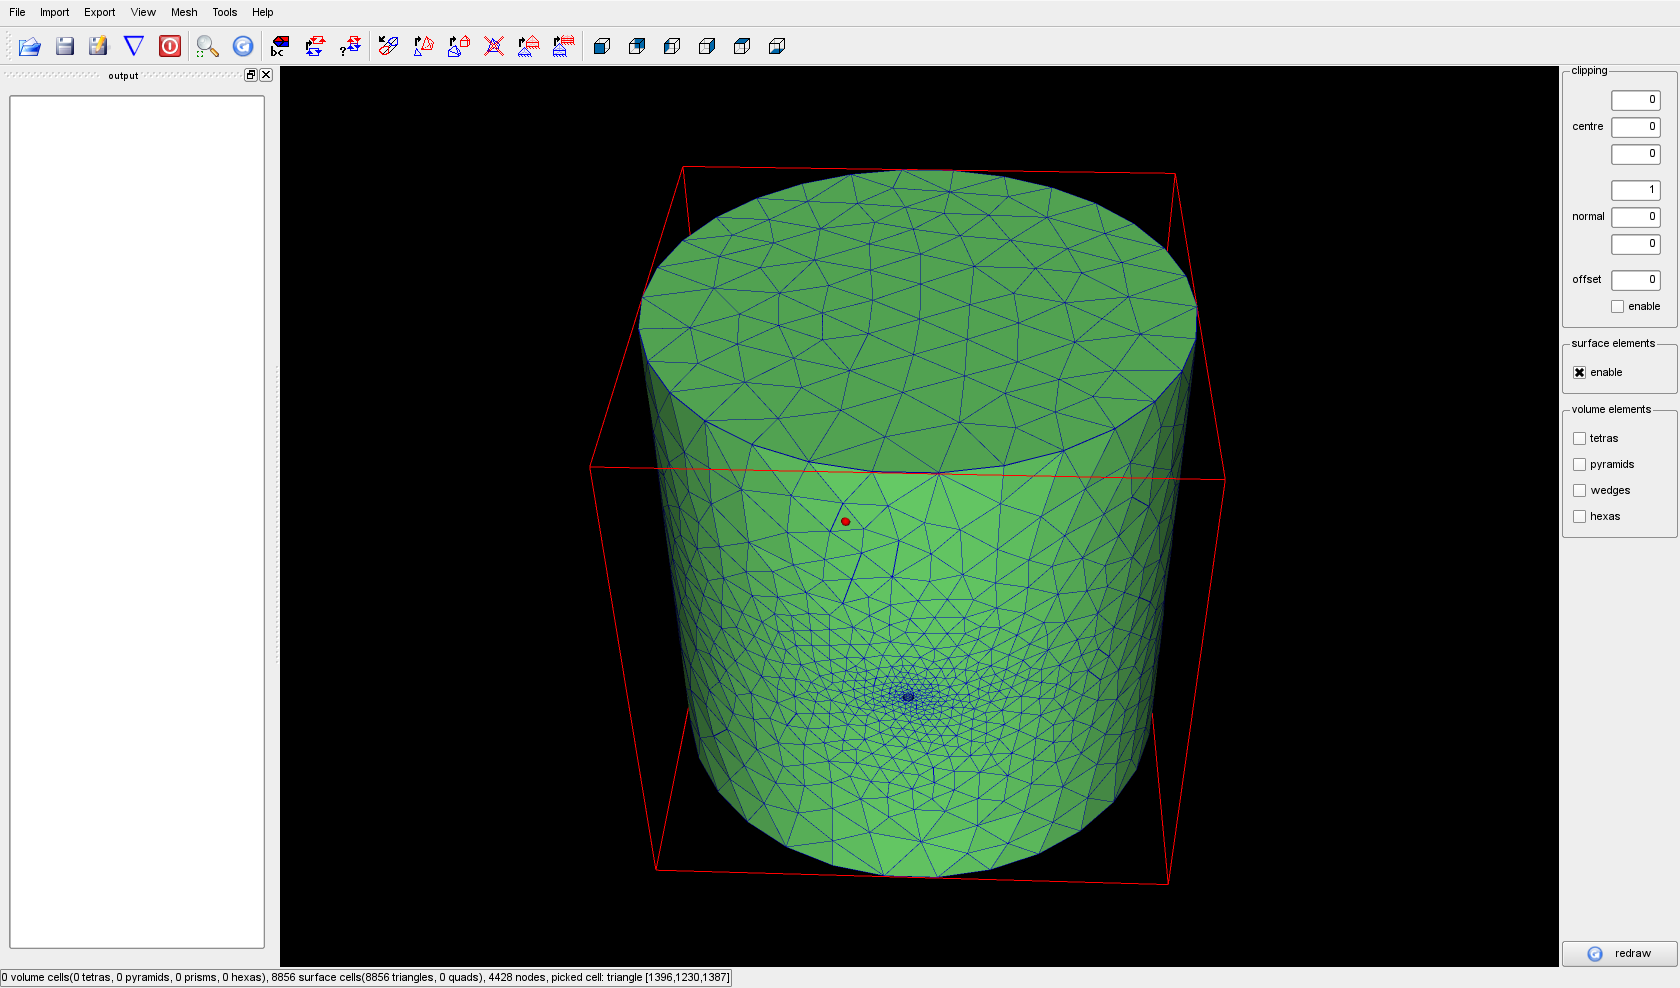
\includegraphics[width=14cm]{figures/tutorials/T1/scr02}
    \par
  \end{centering}
  \caption{After picking a face}
  \label{fig:T1_scr02}
\end{figure}

\begin{figure}
  \begin{centering}
    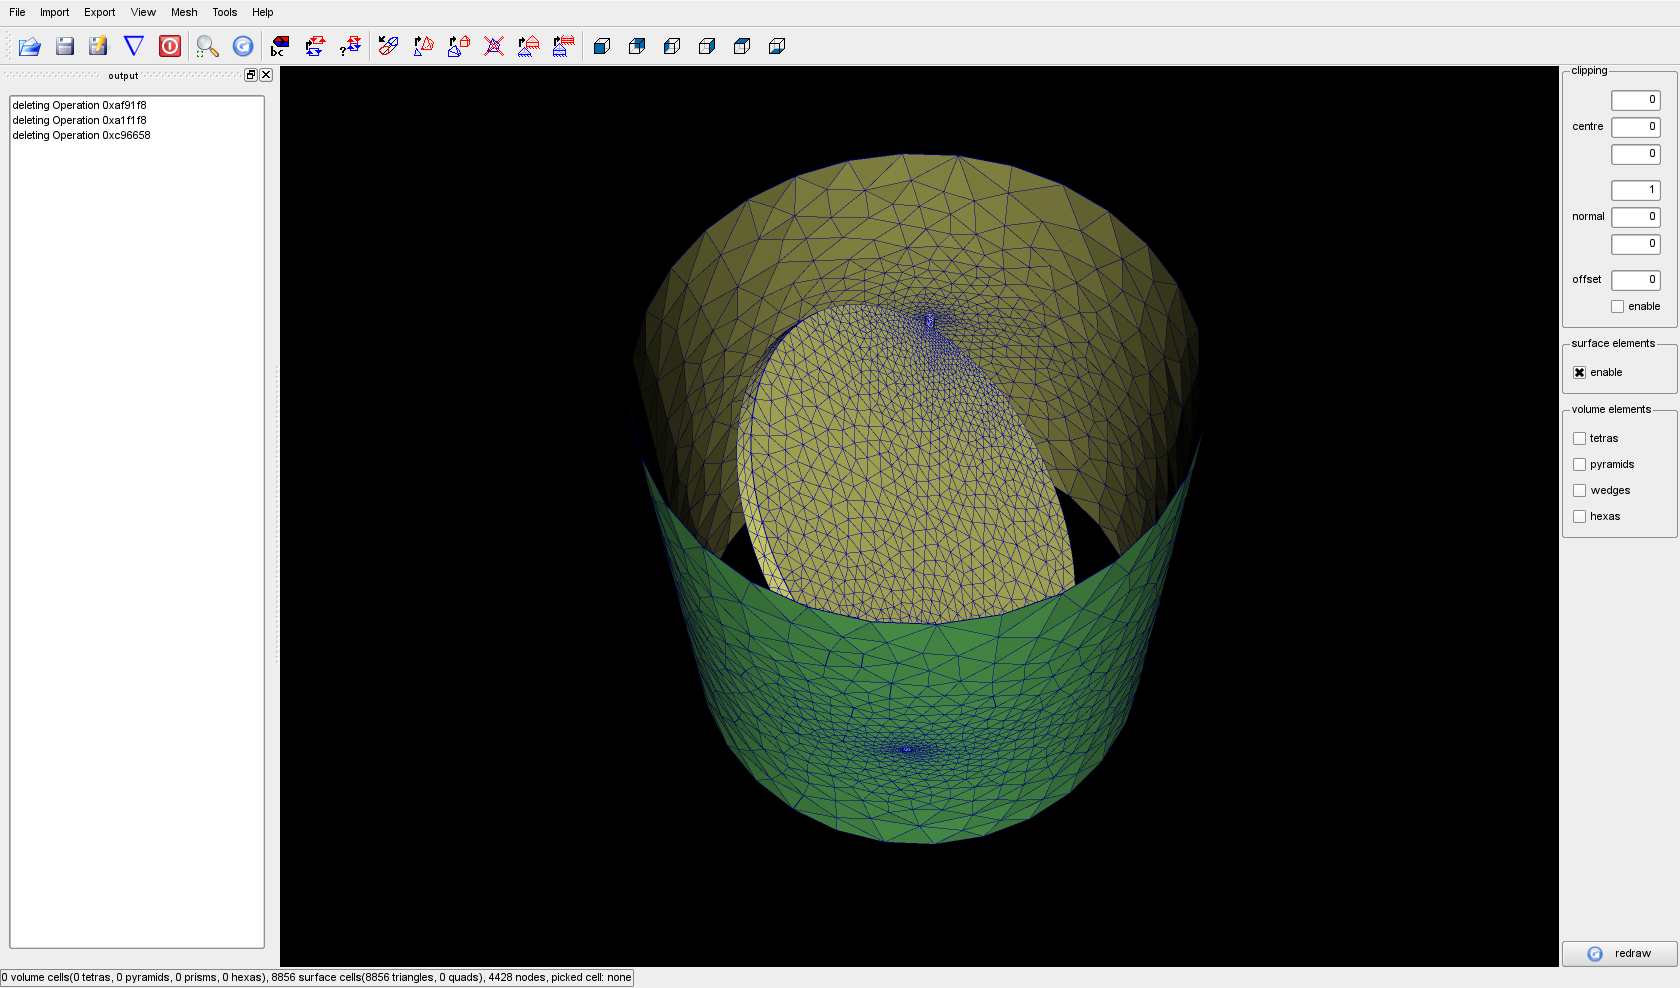
\includegraphics[width=14cm]{figures/tutorials/T1/scr03}
    \par
  \end{centering}
  \caption{Physical walls for prismatic boundary layer}
  \label{fig:T1_scr03}
\end{figure}

\clearpage
\subsubsection{Create Volume Mesh}
Creating a first volume mesh, including the boundary layer, is fairly easy now. First choose

\menu{View \arr boundary codes}
 
and select the boundary conditions 1 and 2, because these represent the physical walls of the geometry. You should now have something similar to figure \ref{fig:T1_scr03}. To create the grid, simply select

\menu{Mesh \arr create prismatic boundary layer}, 

select the boundary conditions 1 and 2 and click {}``OK''. You can watch the progress in the output window on the left side of the screen. This output window can be detached, moved somewhere else, or hidden completely. \eg indicates that it is busy in the status line at the bottom of the window. After \eg has finished you can select {}``tetras'' and {}``wedges'' from
the available options on the right side of \eg's main window. In order to see inside you should also enable the clipping options. The origin of the clipping plane can be set to (0,0,0) and the normal vector to (0,0,-1). If you now select to view only boundary condition 1 and choose

\menu{View \arr redraw}
 
your screen should look similar to figure \ref{fig:T1_scr04}. To get a nice tetrahedral part of the grid it is advisable to execute

\menu{Mesh \arr create improve volume mesh (NETGEN)}

once or twice. The mesh size distribution is not ideal for the first run of NETGEN. \eg uses an existing volume grid to compute a mesh size distribution and uses this as input for the next call of NETGEN. Normally you get a rather coarse tetrahedral grid together with the prismatic layer. The next call will produce a grid that might be somewhat too fine. Starting from the second call of

\menu{Mesh \arr create improve volume mesh (NETGEN)}
 
the grid should look rather nice (see figure \ref{fig:T1_scr04}).

\begin{figure}
  \begin{centering}
    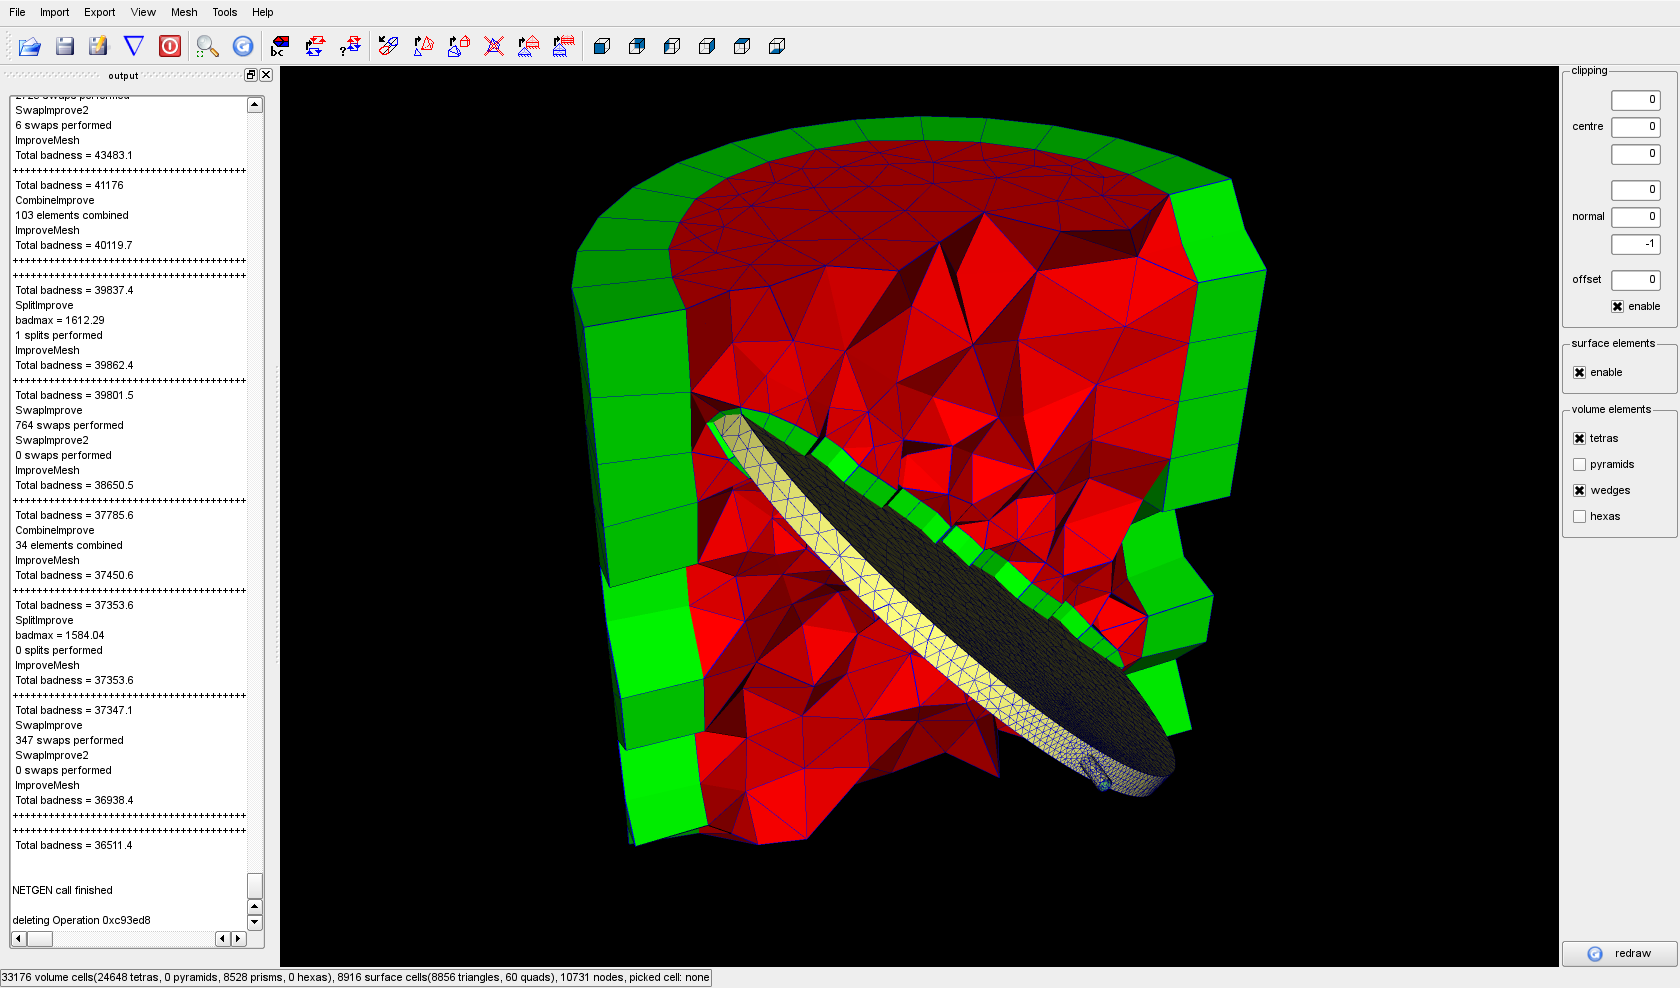
\includegraphics[width=14cm]{figures/tutorials/T1/scr04}
    \par
  \end{centering}
  \caption{First volume grid}
  \label{fig:T1_scr04}
\end{figure}

\clearpage
\subsubsection{Refining the Boundary-Layer}
At the moment the boundary layer consists of a single layer of prisms. Refining the boundary layer is a straightforward process. 

\important
{
  Save the grid with the refined boundary layer to
  a different file name, or don't save it at all (just export). At the
  moment the refinement cannot be reversed and thus the grid spacing
  cannot be changed. To do this, load the file with the initial one-layer
  boundary layer and refine again.
}

To refine the boundary layer, choose

\menu{Mesh \arr divide prismatic boundary layer}.
\begin{figure}
  \begin{centering}
    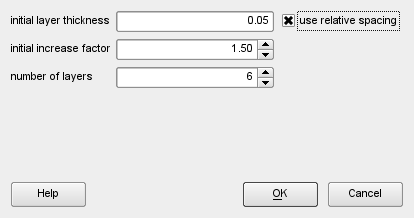
\includegraphics[width=84mm]{figures/tutorials/T1/scr05}
    \par
  \end{centering}
  \caption{Parameters for boundary layer}
  \label{fig:T1_scr05}
\end{figure}

A small pop-up dialogue appears, where you can enter how many layers and how to space them. Relative spacing means, that the initial step size (on the wall) is a fraction of the average local edge length around a node. Absolute spacing uses a fixed distance for all first layer prisms; this will lead to a first layer of prisms which is parallel to the wall. Not all step sizes are possible and \eg will issue a warning if it cannot refine your boundary layer. For this tutorial the settings in figure \ref{fig:T1_scr05} should result in a decent boundary layer mesh.

\clearpage
\subsubsection{Applying a few Simple Modifications}
\eg offers the possibility to modify the grid by extruding certain boundaries. First we will add a pipe bend by applying a rotational extrusion to the upper boundary (code 3). Afterwards we will add straight sections for the in-flow and out-flow boundaries with the help of a normal extrusion. Please select

\menu{Mesh \arr extrusion}

and enter the parameters exactly as shown in figure \ref{fig:T1_scr06}. After clicking OK you should get a grid like the one shown in figure \ref{fig:T1_scr07}. The extrusion adds a new boundary code (5) which needs to be enabled with

\menu{View \arr boundary codes}

in order to view the newly created geometry. The layer height in figure \ref{fig:T1_scr06} corresponds to an angle in degrees for a rotational extrusion. To extend the pipe at the inlet a normal extrusion with the parameters from figure \ref{fig:T1_scr08} shall be used. If you do the same for boundary code 4 the grid should look like in figure \ref{fig:T1_scr09}. To simplify the later setup of a simulation it is advisable to reset the newly created boundary codes (5,6,8) to the initially set value of 2 for the pipe.

\begin{figure}
  \begin{centering}
    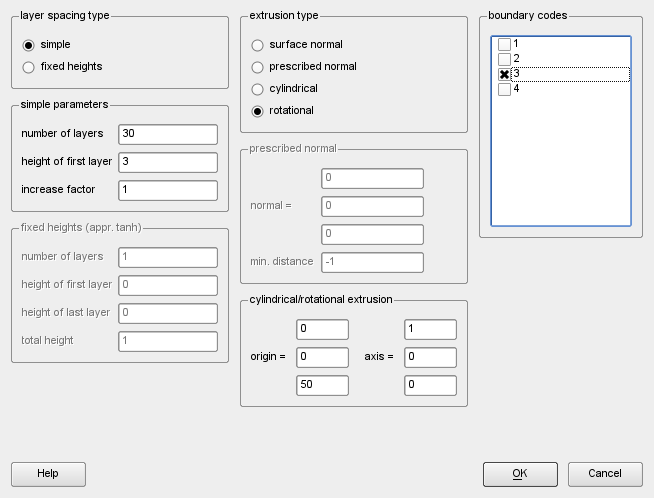
\includegraphics[width=132mm]{figures/tutorials/T1/scr06}
    \par
  \end{centering}
  \caption{Parameters for rotational extrusion}
  \label{fig:T1_scr06}
\end{figure}
\begin{figure}
  \begin{centering}
    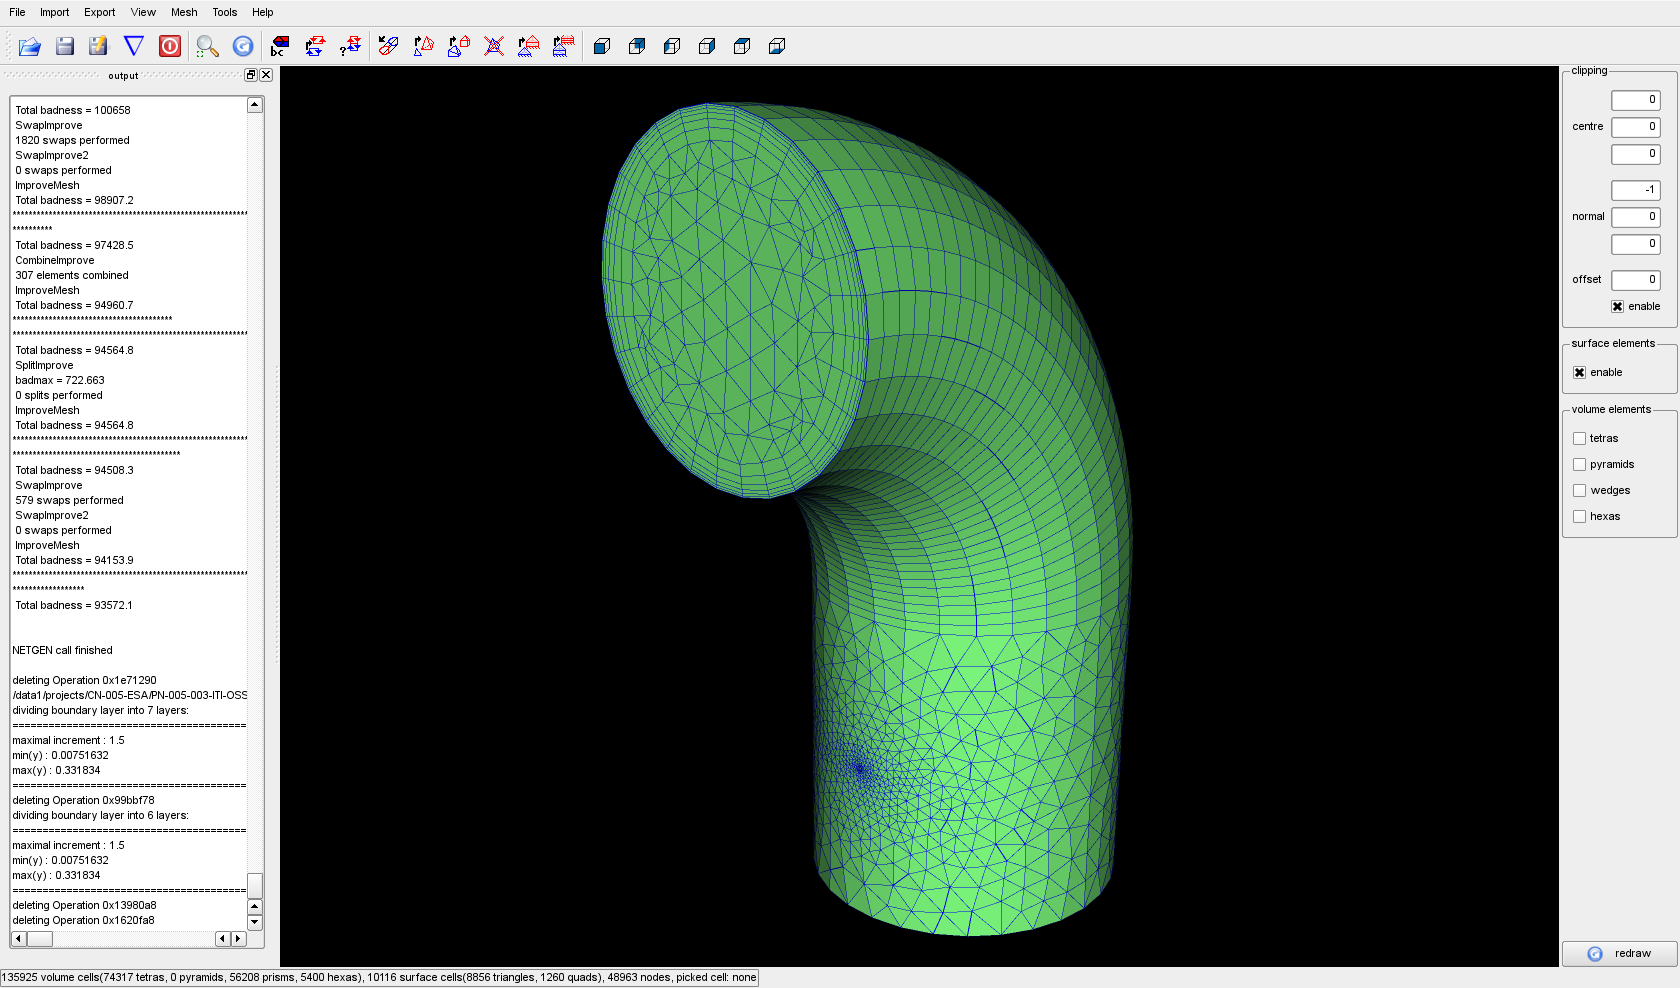
\includegraphics[width=14cm]{figures/tutorials/T1/scr07}
    \par
  \end{centering}
  \caption{Grid after rotational extrusion}
  \label{fig:T1_scr07}
\end{figure}
\begin{figure}
  \begin{centering}
    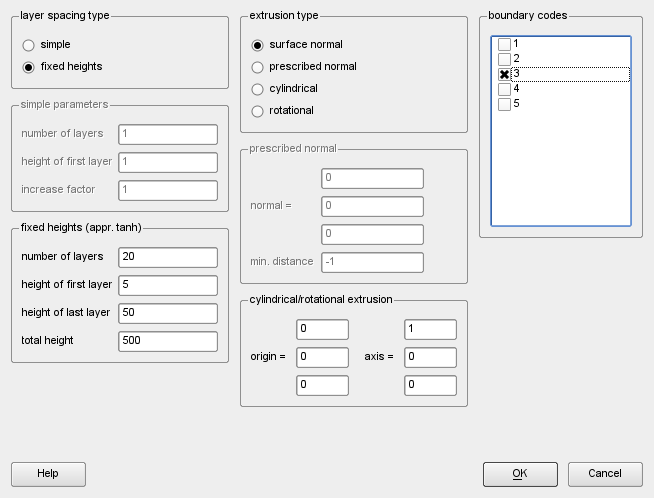
\includegraphics[width=132mm]{figures/tutorials/T1/scr08}
    \par
  \end{centering}
  \caption{Parameters for normal extrusion}
  \label{fig:T1_scr08}
\end{figure}
\begin{figure}
  \begin{centering}
    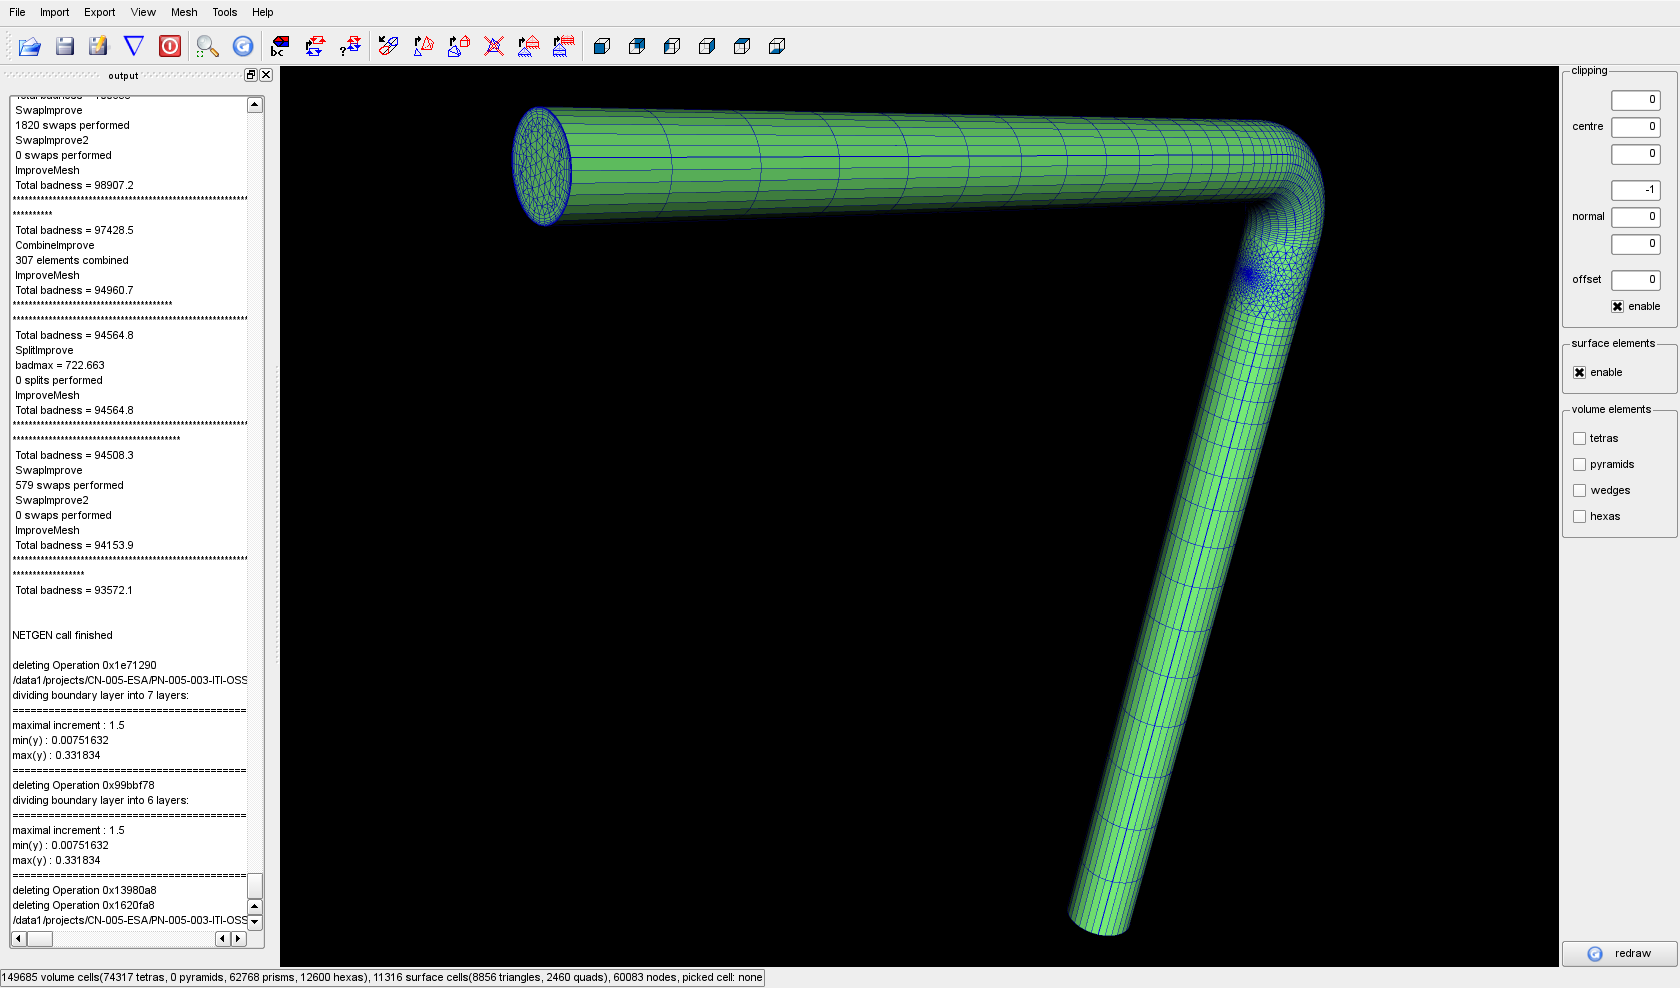
\includegraphics[width=14cm]{figures/tutorials/T1/scr09}
    \par
  \end{centering}
  \caption{Grid after normal extrusion}
  \label{fig:T1_scr09}
\end{figure}
\clearpage

\subsubsection{Export the Grid to \foam}
Please select

\menu{Tools \arr edit boundary conditions}

and edit the boundary names and types according to figure \ref{fig:T1_scr10}. You can export the mesh using:

\menu{Export \arr OpenFOAM \arr  OpenFOAM}.

This will prompt you for an \foam case directory and the mesh will be directly imported to the \foam format, using the boundary names and types you have defined earlier.

\important
{
  OpenFOAM's checkMesh utility might report a bad mesh
  in case of very thin prisms. A good strategy is to export the mesh
  before the boundary layer is refined, run the checkMesh utility, and
  then - if everything looks alright - refine the boundary layer.
}
\begin{figure}
  \begin{centering}
    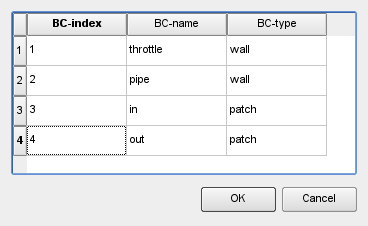
\includegraphics[width=74mm]{figures/tutorials/T1/scr10}
    \par
  \end{centering}
  \caption{Editing the boundary conditions}
  \label{fig:T1_scr10}
\end{figure}

\chapter{Background}

\section{Settings}

\subsection{Feature angle}
The feature angle is used to determine when an edge is a "feature edge", i.e. on the border of a "flat" surface.
A feature edge occurs when the angle between the two surface normals of a polygon sharing an edge is greater than the FeatureAngle.

Those feature edges delimit the area which will be set to the given boundary code.

\begin{figure}
  \begin{centering}
    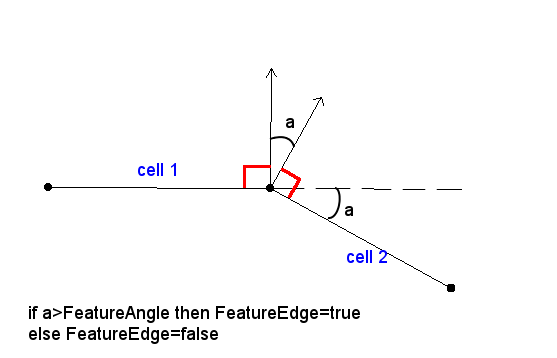
\includegraphics[width=14cm]{figures/featureangle4}
    \par
  \end{centering}
  \caption{The feature angle}
  \label{fig:featureangle4}
\end{figure}

Consider figure \ref{fig:featureangle4}: If you picked cell 1 and chose a feature angle greater than "a", cell 1 and cell 2 will be set to the same boundary code. Otherwise not.

\section{Technical Details}

\subsection{Mesh data structures}

\subsubsection{Cells}

\subsubsection{Local cells}
Depends on:
\begin{itemize}
 \item cells
\end{itemize}

\subsubsection{Nodes}
Depends on:
\begin{itemize}
 \item cells
\end{itemize}

\subsubsection{Local nodes}
Depends on:
\begin{itemize}
 \item cells
 \item nodes
\end{itemize}

\subsubsection{N2N (node to node)}
Depends on:
\begin{itemize}
 \item cells
 \item nodes
 \item local nodes
\end{itemize}

\subsubsection{N2C (node to cell)}
Depends on:
\begin{itemize}
 \item cells
 \item nodes
 \item local nodes
\end{itemize}

\subsubsection{C2C (cell to cell)}
Depends on:
\begin{itemize}
 \item cells
\end{itemize}



\subsection{Initial Boundary Layer Generation}

\subsection{Mesh-Smoothing}

\subsection{Using NETGEN for Tetra-Meshing}


\section{Element Numbering}

\begin{figure}
  \begin{centering}
    \begin{tabular}{>{\centering}m{4cm}>{\raggedright}m{5cm}}
      \vspace{10mm}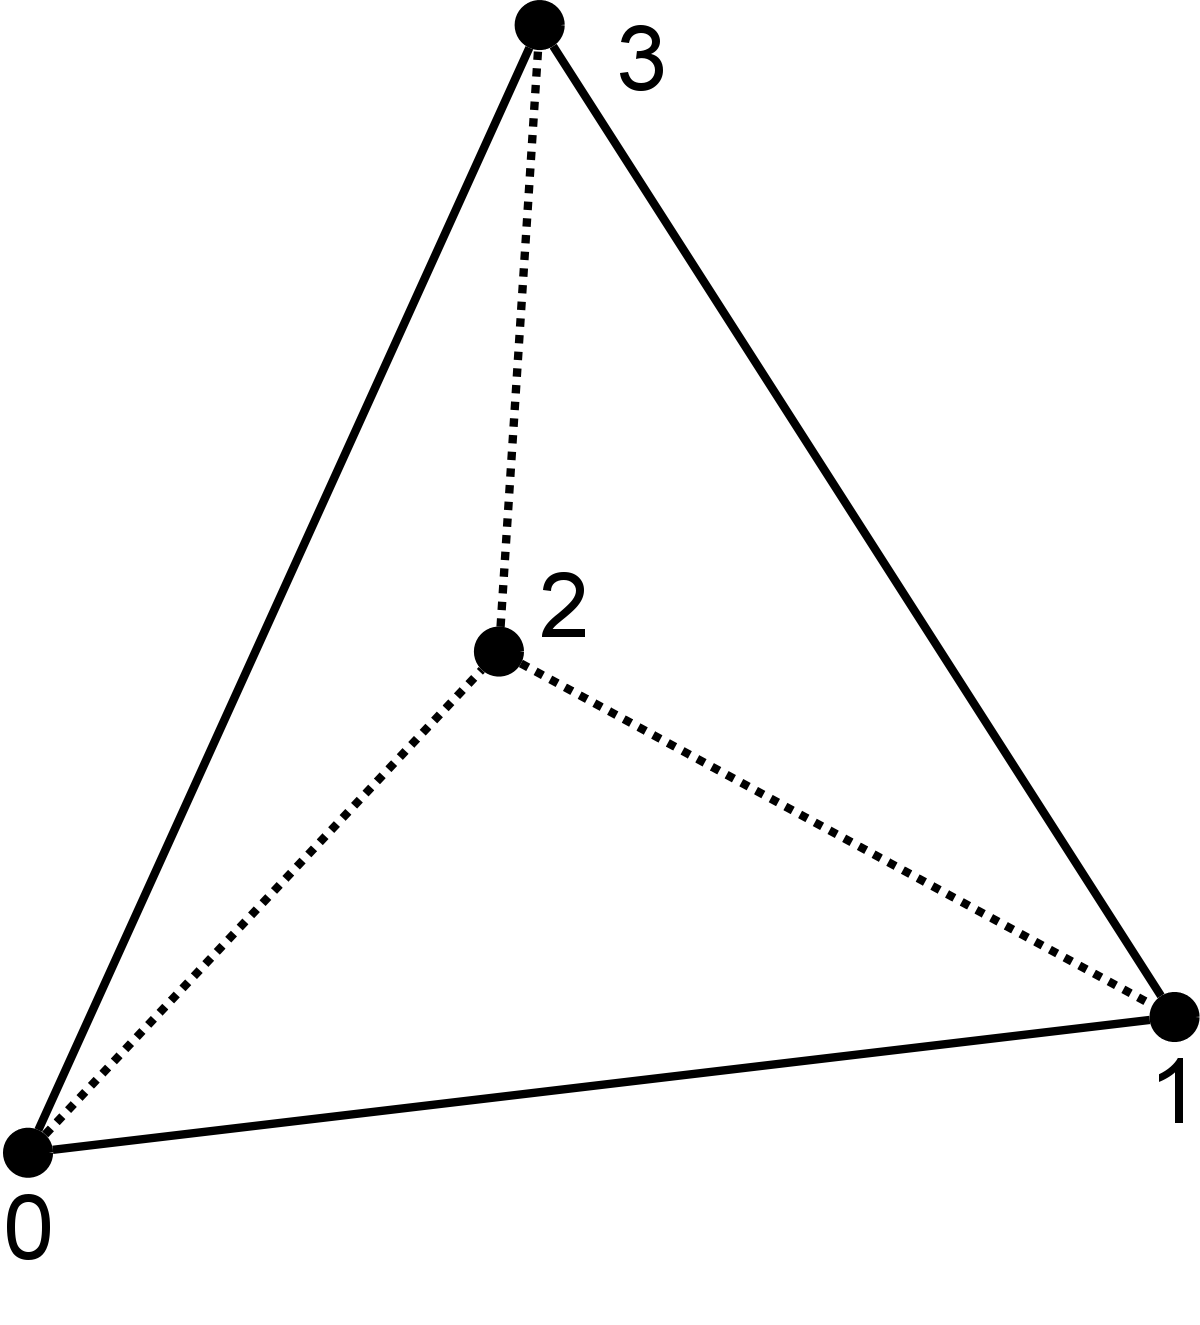
\includegraphics[width=3cm]{figures/Tetra}
      &
      \begin{tabular}{cc|cc}
        \multicolumn{2}{c|}
        {
          faces
        } 
        & 
        \multicolumn{2}{c}
        {
          edges
        }
        \tabularnewline
        \hline
        0 & 2,1,0 & 0 & 0,1 \\
        1 & 1,3,0 & 1 & 0,2 \\
        2 & 3,2,0 & 2 & 0,3 \\
        3 & 2,3,1 & 3 & 1,2 \\
          &       & 4 & 1,3 \\
          &       & 5 & 2,3 \\
      \end{tabular}
    \end{tabular}
    \par
    \end{centering}
  \caption{Tetrahedron}
  \label{fig:tetra}
\end{figure}

\begin{figure}
  \begin{centering}
    \begin{tabular}{>{\centering}m{4cm}>{\raggedright}m{5cm}}
      \vspace{10mm}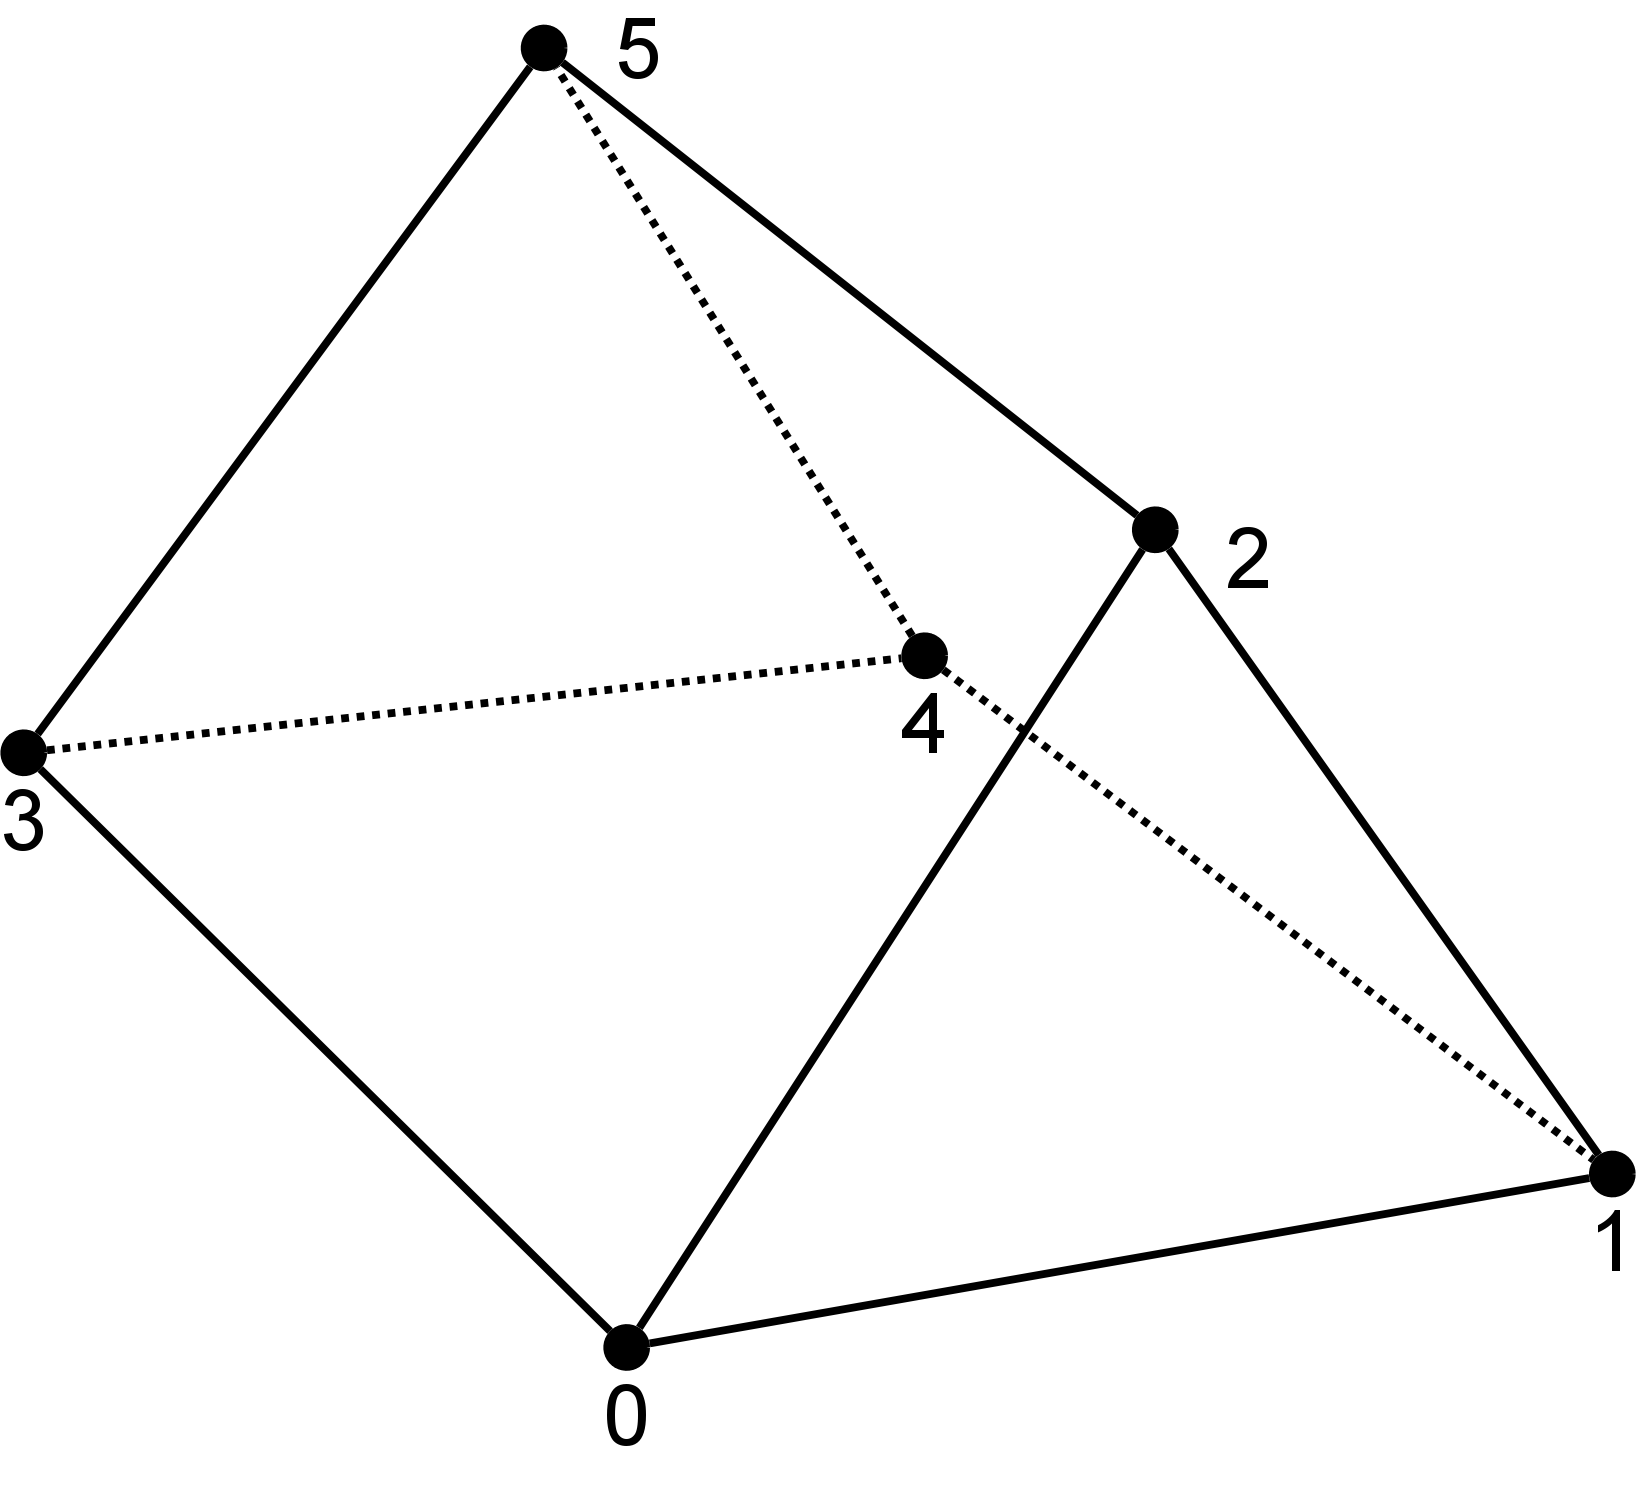
\includegraphics[width=3cm]{figures/Wedge}
      &
      \begin{tabular}{cc|cc}
        \multicolumn{2}{c|}
        {
          faces
        } 
        & 
        \multicolumn{2}{c}
        {
          edges
        }
        \tabularnewline
        \hline
        0 & 0,1,2   & 0 & 0,1 \\
        1 & 3,5,4   & 1 & 0,2 \\
        2 & 3,4,1,0 & 2 & 0,3 \\
        3 & 1,4,5,2 & 3 & 1,2 \\
        4 & 0,2,5,3 & 4 & 1,4 \\
          &         & 5 & 2,5 \\
          &         & 6 & 3,4 \\
          &         & 7 & 3,5 \\
          &         & 8 & 4,5 \\
      \end{tabular}
    \end{tabular}
    \par
    \end{centering}
  \caption{Wedge/Prism}
  \label{fig:tetra}
\end{figure}

\begin{figure}
  \begin{centering}
    \begin{tabular}{>{\centering}m{4cm}>{\raggedright}m{5cm}}
      \vspace{10mm}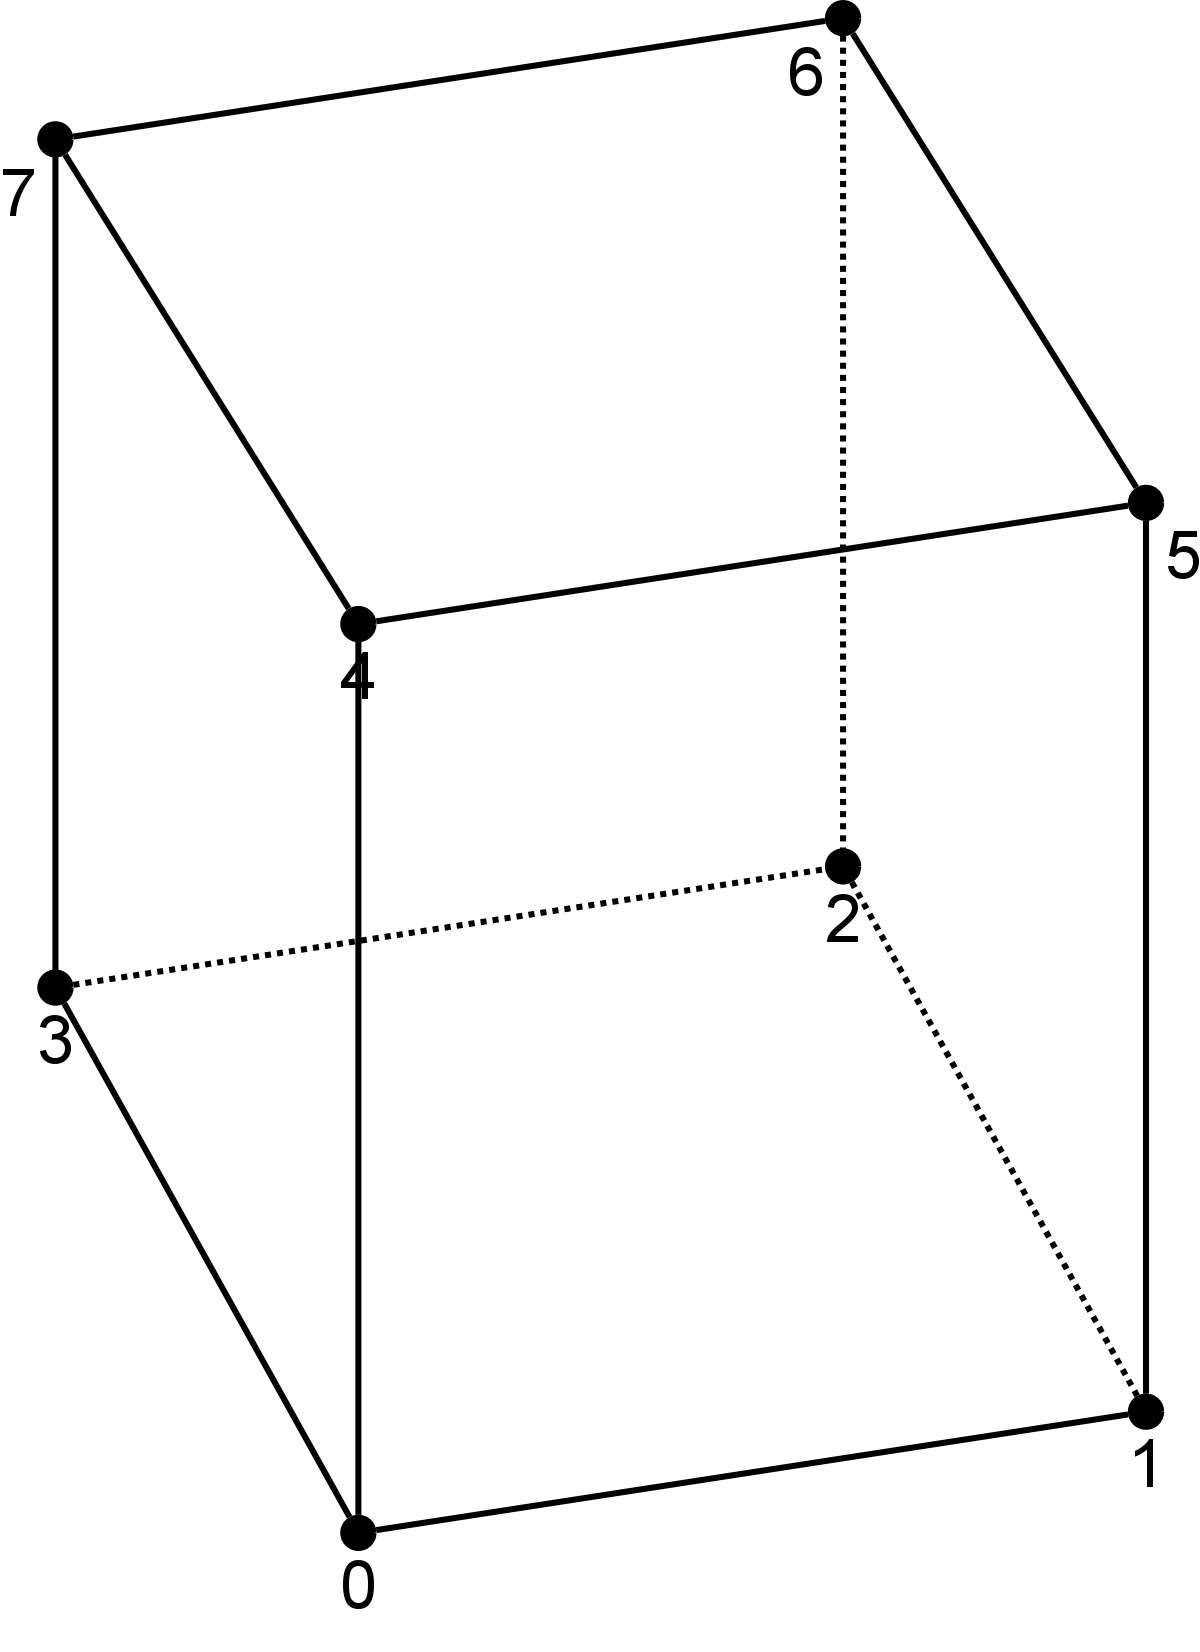
\includegraphics[width=3cm]{figures/Hexa}
      &
      \begin{tabular}{cc|cc}
        \multicolumn{2}{c|}
        {
          faces
        } 
        & 
        \multicolumn{2}{c}
        {
          edges
        }
        \tabularnewline
        \hline
        0 & 0,3,2,1 & 0  & 0,1 \\
        1 & 4,5,6,7 & 1  & 0,3 \\
        2 & 0,1,5,4 & 2  & 0,4 \\
        3 & 3,7,6,2 & 3  & 1,2 \\
        4 & 0,4,7,3 & 4  & 1,5 \\
        5 & 1,2,6,5 & 5  & 2,3 \\
          &         & 6  & 2,6 \\
          &         & 7  & 3,7 \\
          &         & 8  & 4,5 \\
          &         & 9  & 4,7 \\
          &         & 10 & 5,6 \\
          &         & 11 & 6,7 \\
      \end{tabular}
    \end{tabular}
    \par
    \end{centering}
  \caption{Hexahedron}
  \label{fig:tetra}
\end{figure}

\section{Planned Developments}


\appendix

\chapter{GNU Free Documentation License}

 \begin{center}

       Version 1.2, November 2002


 Copyright \copyright{} 2000,2001,2002  Free Software Foundation, Inc.
 
 \bigskip
 
     51 Franklin St, Fifth Floor, Boston, MA  02110-1301  USA
  
 \bigskip
 
 Everyone is permitted to copy and distribute verbatim copies
 of this license document, but changing it is not allowed.
\end{center}


{\bf\large Preamble}

The purpose of this License is to make a manual, textbook, or other
functional and useful document ``free'' in the sense of freedom: to
assure everyone the effective freedom to copy and redistribute it,
with or without modifying it, either commercially or noncommercially.
Secondarily, this License preserves for the author and publisher a way
to get credit for their work, while not being considered responsible
for modifications made by others.

This License is a kind of ``copyleft'', which means that derivative
works of the document must themselves be free in the same sense.  It
complements the GNU General Public License, which is a copyleft
license designed for free software.

We have designed this License in order to use it for manuals for free
software, because free software needs free documentation: a free
program should come with manuals providing the same freedoms that the
software does.  But this License is not limited to software manuals;
it can be used for any textual work, regardless of subject matter or
whether it is published as a printed book.  We recommend this License
principally for works whose purpose is instruction or reference.


{\Large\bf 1. APPLICABILITY AND DEFINITIONS\par}

This License applies to any manual or other work, in any medium, that
contains a notice placed by the copyright holder saying it can be
distributed under the terms of this License.  Such a notice grants a
world-wide, royalty-free license, unlimited in duration, to use that
work under the conditions stated herein.  The ``\textbf{Document}'', below,
refers to any such manual or work.  Any member of the public is a
licensee, and is addressed as ``\textbf{you}''.  You accept the license if you
copy, modify or distribute the work in a way requiring permission
under copyright law.

A ``\textbf{Modified Version}'' of the Document means any work containing the
Document or a portion of it, either copied verbatim, or with
modifications and/or translated into another language.

A ``\textbf{Secondary Section}'' is a named appendix or a front-matter section of
the Document that deals exclusively with the relationship of the
publishers or authors of the Document to the Document's overall subject
(or to related matters) and contains nothing that could fall directly
within that overall subject.  (Thus, if the Document is in part a
textbook of mathematics, a Secondary Section may not explain any
mathematics.)  The relationship could be a matter of historical
connection with the subject or with related matters, or of legal,
commercial, philosophical, ethical or political position regarding
them.

The ``\textbf{Invariant Sections}'' are certain Secondary Sections whose titles
are designated, as being those of Invariant Sections, in the notice
that says that the Document is released under this License.  If a
section does not fit the above definition of Secondary then it is not
allowed to be designated as Invariant.  The Document may contain zero
Invariant Sections.  If the Document does not identify any Invariant
Sections then there are none.

The ``\textbf{Cover Texts}'' are certain short passages of text that are listed,
as Front-Cover Texts or Back-Cover Texts, in the notice that says that
the Document is released under this License.  A Front-Cover Text may
be at most 5 words, and a Back-Cover Text may be at most 25 words.

A ``\textbf{Transparent}'' copy of the Document means a machine-readable copy,
represented in a format whose specification is available to the
general public, that is suitable for revising the document
straightforwardly with generic text editors or (for images composed of
pixels) generic paint programs or (for drawings) some widely available
drawing editor, and that is suitable for input to text formatters or
for automatic translation to a variety of formats suitable for input
to text formatters.  A copy made in an otherwise Transparent file
format whose markup, or absence of markup, has been arranged to thwart
or discourage subsequent modification by readers is not Transparent.
An image format is not Transparent if used for any substantial amount
of text.  A copy that is not ``Transparent'' is called ``\textbf{Opaque}''.

Examples of suitable formats for Transparent copies include plain
ASCII without markup, Texinfo input format, LaTeX input format, SGML
or XML using a publicly available DTD, and standard-conforming simple
HTML, PostScript or PDF designed for human modification.  Examples of
transparent image formats include PNG, XCF and JPG.  Opaque formats
include proprietary formats that can be read and edited only by
proprietary word processors, SGML or XML for which the DTD and/or
processing tools are not generally available, and the
machine-generated HTML, PostScript or PDF produced by some word
processors for output purposes only.

The ``\textbf{Title Page}'' means, for a printed book, the title page itself,
plus such following pages as are needed to hold, legibly, the material
this License requires to appear in the title page.  For works in
formats which do not have any title page as such, ``Title Page'' means
the text near the most prominent appearance of the work's title,
preceding the beginning of the body of the text.

A section ``\textbf{Entitled XYZ}'' means a named subunit of the Document whose
title either is precisely XYZ or contains XYZ in parentheses following
text that translates XYZ in another language.  (Here XYZ stands for a
specific section name mentioned below, such as ``\textbf{Acknowledgements}'',
``\textbf{Dedications}'', ``\textbf{Endorsements}'', or ``\textbf{History}''.)  
To ``\textbf{Preserve the Title}''
of such a section when you modify the Document means that it remains a
section ``Entitled XYZ'' according to this definition.

The Document may include Warranty Disclaimers next to the notice which
states that this License applies to the Document.  These Warranty
Disclaimers are considered to be included by reference in this
License, but only as regards disclaiming warranties: any other
implication that these Warranty Disclaimers may have is void and has
no effect on the meaning of this License.


{\Large\bf 2. VERBATIM COPYING\par}

You may copy and distribute the Document in any medium, either
commercially or noncommercially, provided that this License, the
copyright notices, and the license notice saying this License applies
to the Document are reproduced in all copies, and that you add no other
conditions whatsoever to those of this License.  You may not use
technical measures to obstruct or control the reading or further
copying of the copies you make or distribute.  However, you may accept
compensation in exchange for copies.  If you distribute a large enough
number of copies you must also follow the conditions in section~3.

You may also lend copies, under the same conditions stated above, and
you may publicly display copies.


{\Large\bf 3. COPYING IN QUANTITY\par}


If you publish printed copies (or copies in media that commonly have
printed covers) of the Document, numbering more than 100, and the
Document's license notice requires Cover Texts, you must enclose the
copies in covers that carry, clearly and legibly, all these Cover
Texts: Front-Cover Texts on the front cover, and Back-Cover Texts on
the back cover.  Both covers must also clearly and legibly identify
you as the publisher of these copies.  The front cover must present
the full title with all words of the title equally prominent and
visible.  You may add other material on the covers in addition.
Copying with changes limited to the covers, as long as they preserve
the title of the Document and satisfy these conditions, can be treated
as verbatim copying in other respects.

If the required texts for either cover are too voluminous to fit
legibly, you should put the first ones listed (as many as fit
reasonably) on the actual cover, and continue the rest onto adjacent
pages.

If you publish or distribute Opaque copies of the Document numbering
more than 100, you must either include a machine-readable Transparent
copy along with each Opaque copy, or state in or with each Opaque copy
a computer-network location from which the general network-using
public has access to download using public-standard network protocols
a complete Transparent copy of the Document, free of added material.
If you use the latter option, you must take reasonably prudent steps,
when you begin distribution of Opaque copies in quantity, to ensure
that this Transparent copy will remain thus accessible at the stated
location until at least one year after the last time you distribute an
Opaque copy (directly or through your agents or retailers) of that
edition to the public.

It is requested, but not required, that you contact the authors of the
Document well before redistributing any large number of copies, to give
them a chance to provide you with an updated version of the Document.


{\Large\bf 4. MODIFICATIONS\par}

You may copy and distribute a Modified Version of the Document under
the conditions of sections 2 and 3 above, provided that you release
the Modified Version under precisely this License, with the Modified
Version filling the role of the Document, thus licensing distribution
and modification of the Modified Version to whoever possesses a copy
of it.  In addition, you must do these things in the Modified Version:

\begin{itemize}
\item[A.] 
   Use in the Title Page (and on the covers, if any) a title distinct
   from that of the Document, and from those of previous versions
   (which should, if there were any, be listed in the History section
   of the Document).  You may use the same title as a previous version
   if the original publisher of that version gives permission.
   
\item[B.]
   List on the Title Page, as authors, one or more persons or entities
   responsible for authorship of the modifications in the Modified
   Version, together with at least five of the principal authors of the
   Document (all of its principal authors, if it has fewer than five),
   unless they release you from this requirement.
   
\item[C.]
   State on the Title page the name of the publisher of the
   Modified Version, as the publisher.
   
\item[D.]
   Preserve all the copyright notices of the Document.
   
\item[E.]
   Add an appropriate copyright notice for your modifications
   adjacent to the other copyright notices.
   
\item[F.]
   Include, immediately after the copyright notices, a license notice
   giving the public permission to use the Modified Version under the
   terms of this License, in the form shown in the Addendum below.
   
\item[G.]
   Preserve in that license notice the full lists of Invariant Sections
   and required Cover Texts given in the Document's license notice.
   
\item[H.]
   Include an unaltered copy of this License.
   
\item[I.]
   Preserve the section Entitled ``History'', Preserve its Title, and add
   to it an item stating at least the title, year, new authors, and
   publisher of the Modified Version as given on the Title Page.  If
   there is no section Entitled ``History'' in the Document, create one
   stating the title, year, authors, and publisher of the Document as
   given on its Title Page, then add an item describing the Modified
   Version as stated in the previous sentence.
   
\item[J.]
   Preserve the network location, if any, given in the Document for
   public access to a Transparent copy of the Document, and likewise
   the network locations given in the Document for previous versions
   it was based on.  These may be placed in the ``History'' section.
   You may omit a network location for a work that was published at
   least four years before the Document itself, or if the original
   publisher of the version it refers to gives permission.
   
\item[K.]
   For any section Entitled ``Acknowledgements'' or ``Dedications'',
   Preserve the Title of the section, and preserve in the section all
   the substance and tone of each of the contributor acknowledgements
   and/or dedications given therein.
   
\item[L.]
   Preserve all the Invariant Sections of the Document,
   unaltered in their text and in their titles.  Section numbers
   or the equivalent are not considered part of the section titles.
   
\item[M.]
   Delete any section Entitled ``Endorsements''.  Such a section
   may not be included in the Modified Version.
   
\item[N.]
   Do not retitle any existing section to be Entitled ``Endorsements''
   or to conflict in title with any Invariant Section.
   
\item[O.]
   Preserve any Warranty Disclaimers.
\end{itemize}

If the Modified Version includes new front-matter sections or
appendices that qualify as Secondary Sections and contain no material
copied from the Document, you may at your option designate some or all
of these sections as invariant.  To do this, add their titles to the
list of Invariant Sections in the Modified Version's license notice.
These titles must be distinct from any other section titles.

You may add a section Entitled ``Endorsements'', provided it contains
nothing but endorsements of your Modified Version by various
parties--for example, statements of peer review or that the text has
been approved by an organization as the authoritative definition of a
standard.

You may add a passage of up to five words as a Front-Cover Text, and a
passage of up to 25 words as a Back-Cover Text, to the end of the list
of Cover Texts in the Modified Version.  Only one passage of
Front-Cover Text and one of Back-Cover Text may be added by (or
through arrangements made by) any one entity.  If the Document already
includes a cover text for the same cover, previously added by you or
by arrangement made by the same entity you are acting on behalf of,
you may not add another; but you may replace the old one, on explicit
permission from the previous publisher that added the old one.

The author(s) and publisher(s) of the Document do not by this License
give permission to use their names for publicity for or to assert or
imply endorsement of any Modified Version.


{\Large\bf 5. COMBINING DOCUMENTS\par}


You may combine the Document with other documents released under this
License, under the terms defined in section~4 above for modified
versions, provided that you include in the combination all of the
Invariant Sections of all of the original documents, unmodified, and
list them all as Invariant Sections of your combined work in its
license notice, and that you preserve all their Warranty Disclaimers.

The combined work need only contain one copy of this License, and
multiple identical Invariant Sections may be replaced with a single
copy.  If there are multiple Invariant Sections with the same name but
different contents, make the title of each such section unique by
adding at the end of it, in parentheses, the name of the original
author or publisher of that section if known, or else a unique number.
Make the same adjustment to the section titles in the list of
Invariant Sections in the license notice of the combined work.

In the combination, you must combine any sections Entitled ``History''
in the various original documents, forming one section Entitled
``History''; likewise combine any sections Entitled ``Acknowledgements'',
and any sections Entitled ``Dedications''.  You must delete all sections
Entitled ``Endorsements''.

{\Large\bf 6. COLLECTIONS OF DOCUMENTS\par}

You may make a collection consisting of the Document and other documents
released under this License, and replace the individual copies of this
License in the various documents with a single copy that is included in
the collection, provided that you follow the rules of this License for
verbatim copying of each of the documents in all other respects.

You may extract a single document from such a collection, and distribute
it individually under this License, provided you insert a copy of this
License into the extracted document, and follow this License in all
other respects regarding verbatim copying of that document.


{\Large\bf 7. AGGREGATION WITH INDEPENDENT WORKS\par}


A compilation of the Document or its derivatives with other separate
and independent documents or works, in or on a volume of a storage or
distribution medium, is called an ``aggregate'' if the copyright
resulting from the compilation is not used to limit the legal rights
of the compilation's users beyond what the individual works permit.
When the Document is included in an aggregate, this License does not
apply to the other works in the aggregate which are not themselves
derivative works of the Document.

If the Cover Text requirement of section~3 is applicable to these
copies of the Document, then if the Document is less than one half of
the entire aggregate, the Document's Cover Texts may be placed on
covers that bracket the Document within the aggregate, or the
electronic equivalent of covers if the Document is in electronic form.
Otherwise they must appear on printed covers that bracket the whole
aggregate.


{\Large\bf 8. TRANSLATION\par}


Translation is considered a kind of modification, so you may
distribute translations of the Document under the terms of section~4.
Replacing Invariant Sections with translations requires special
permission from their copyright holders, but you may include
translations of some or all Invariant Sections in addition to the
original versions of these Invariant Sections.  You may include a
translation of this License, and all the license notices in the
Document, and any Warranty Disclaimers, provided that you also include
the original English version of this License and the original versions
of those notices and disclaimers.  In case of a disagreement between
the translation and the original version of this License or a notice
or disclaimer, the original version will prevail.

If a section in the Document is Entitled ``Acknowledgements'',
``Dedications'', or ``History'', the requirement (section~4) to Preserve
its Title (section~1) will typically require changing the actual
title.


{\Large\bf 9. TERMINATION\par}


You may not copy, modify, sublicense, or distribute the Document except
as expressly provided for under this License.  Any other attempt to
copy, modify, sublicense or distribute the Document is void, and will
automatically terminate your rights under this License.  However,
parties who have received copies, or rights, from you under this
License will not have their licenses terminated so long as such
parties remain in full compliance.


{\Large\bf 10. FUTURE REVISIONS OF THIS LICENSE\par}


The Free Software Foundation may publish new, revised versions
of the GNU Free Documentation License from time to time.  Such new
versions will be similar in spirit to the present version, but may
differ in detail to address new problems or concerns.  See
http://www.gnu.org/copyleft/.

Each version of the License is given a distinguishing version number.
If the Document specifies that a particular numbered version of this
License ``or any later version'' applies to it, you have the option of
following the terms and conditions either of that specified version or
of any later version that has been published (not as a draft) by the
Free Software Foundation.  If the Document does not specify a version
number of this License, you may choose any version ever published (not
as a draft) by the Free Software Foundation.


\addcontentsline{toc}{section}{References}

\begin{flushleft}
\bibliographystyle{plain}
\bibliography{engits}
\par\end{flushleft}

\end{document}

